\section{Clustering}
We now run and compare some clustering algorithm in order to find some structures among the data. First we start with a basic \emph{K-Means}, followed by \emph{Hierarchical clustering techniques} and \emph{DBSCAN}. In the end, we also analyze the behavior of other algorithms, like \emph{Fuzzy C-Means} and \emph{Birch}.

\subsection{Preprocessing}

\begin{wrapfigure}[7]{r}{0.35\textwidth}
\vspace{-20mm}
\centering
\captionsetup{justification=centering}
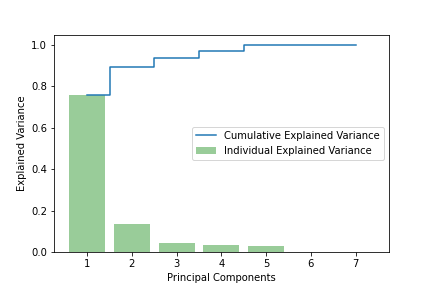
\includegraphics[width=.35\textwidth]{img/clustering/pca.png}
\caption{Explained variance ratio}
\label{fig:pca_img}
\end{wrapfigure}

The data matrix was first standardized and then the two principal components were extracted. The choice was between two and tree principal component since they retain respectively $\sim$0.75 and $\sim$0.89 of the variance of the data.

We selected the two principal components, in this way, we could also have a visual inspection.

\subsection{K-Means}
\begin{wrapfigure}[11]{l}{.4\textwidth}
    \centering
    \captionsetup{justification=centering}
    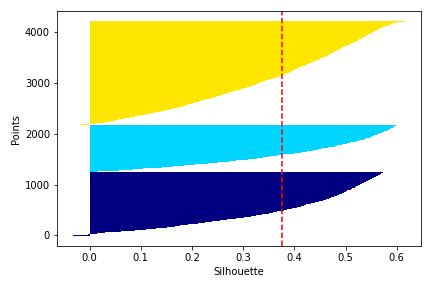
\includegraphics[width=.3\textwidth]{img/clustering/sil_tot.png}
    \caption{Silhouette score\\ for each data point}
    \label{fig:silhouette}
\end{wrapfigure}
The algorithm runs for $K$ ranging from \emph{2} to \emph{15} clusters. For each iteration the SSE and the average silhouette value were computed.

By looking at the plots in Figure \ref{fig:km_metrics}, we can see that there isn't a prominent \emph{elbow shape}, so we needed the analysis of more metrics to get the optimal number of clusters. By inspecting the silhouette score, it is possible to see that it has its maximum for $K = 2$, followed by $K = 3$. In conclusion, we opted for 3 clusters, to get a trade off between high silhouette and low SSE.

\begin{figure}[h!]
     \captionsetup{justification=centering}		
     \centering
     \begin{subfigure}{0.49\textwidth}
         \centering
	 \captionsetup{type=figure}
         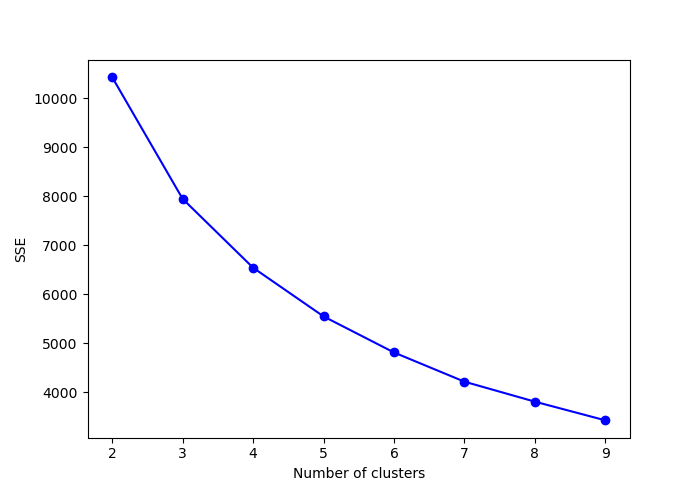
\includegraphics[width=\textwidth]{img/clustering/sse.png}
         \caption{SSE}
         \label{fig:sse}
     \end{subfigure}
     \begin{subfigure}{0.49\textwidth}
         \centering
         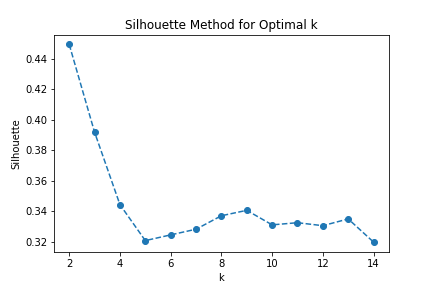
\includegraphics[width=\textwidth]{img/clustering/sil.png}
         \caption{Average silhouette}
         \label{fig:sil}
     \end{subfigure}
     \caption{\emph{K-Means} metrics}
    \label{fig:km_metrics}
\end{figure}

The resulting clusters have a comparable number of points. In particular, \emph{Cluster 2} has \textbf{2006} points, \emph{Cluster 1} \textbf{1440} and \emph{Cluster 0} \textbf{760}.\\
In Figure \ref{fig:silhouette}, we can see the plot of the Silhouette score, where each different color represents a different cluster, and the dotted red line is the average silhouette score. In particular we have that \emph{Cluster 0} has a silhouette of \emph{0.39}, \emph{0.40} for \emph{Cluster 1} and \emph{0.35} for \emph{Cluster 2}, with an overall average silhouette of \emph{0.39}. We see that a small fraction of points in \emph{Cluster 0} have a negative value but overall the Silhouette suggests a good clustering.

In Figure \ref{fig:km_clusters}, we can appreciate the results of the algorithm, where we can see that the clusters are well separated from one another.\\
The similarity matrix (Figure \ref{fig:sim_heatmap}) shows the affinity of elements inside a cluster; we can see that the results are pretty good. Customers within the same cluster are similar, where similarity between two customers is measured using $e^{-d}$, where $d$ is the eucledian distance.\\
The plot in Figure \ref{fig:cluster_avg} shows the average values for each attribute divided by the clusters. In particular, it is possible to see that \emph{Cluster 0} contains the most frequent and spending customers, followed by \emph{Cluster 1} and \emph{Cluster 2}.

\begin{figure}[h!]
    \centering
    \captionsetup{justification=centering}
    \begin{subfigure}{0.32\textwidth}
        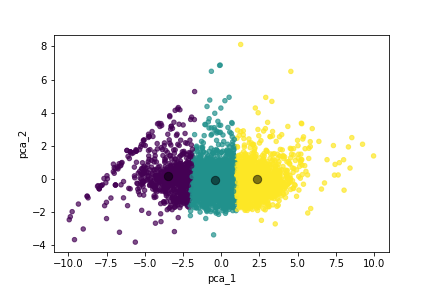
\includegraphics[width=\textwidth]{img/clustering/km_clusters.png}
        \caption{Clustering result}
        \label{fig:km_clusters}
    \end{subfigure}
    \begin{subfigure}{0.32\textwidth}
        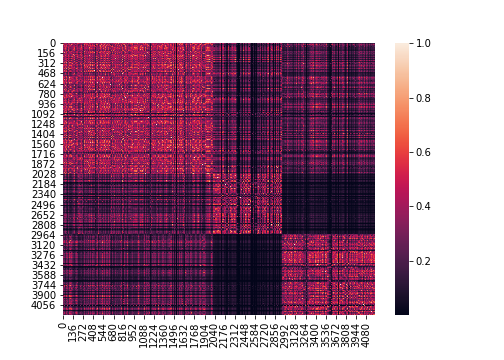
\includegraphics[width=\textwidth]{img/clustering/sim_heatmap.png}
        \caption{Similarity heatmap}
        \label{fig:sim_heatmap}
    \end{subfigure}
    \begin{subfigure}{0.32\textwidth}
        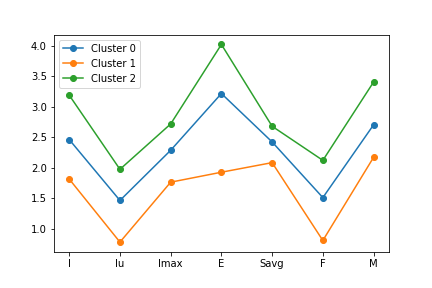
\includegraphics[width=\textwidth]{img/clustering/cluster_avg.png}
	\caption{Average values\\ per cluster}
        \label{fig:cluster_avg}
    \end{subfigure}
\caption{K-Means}
\end{figure}

\vspace{-5mm}
\subsection{Hierarchical clustering}
We used different kinds of algorithm: \emph{Complete Link}, \emph{Single Link}, \emph{Ward Link} and \emph{Average Link}. By looking at the dendograms in Figure \ref{fig:dendograms}, if we cut the tree by selecting two or three clusters, we can see that \emph{Single Link} and \emph{Average Link} generate an unbalanced clustering, leaving the last merges between a large cluster and a small one, in a case even a singleton. The most balanced results are obtained with \emph{Ward Link} and \emph{Complete Link}.

\begin{figure}[h!]
    \centering
	\vspace*{-0.3cm}
    \begin{subfigure}{0.49\textwidth}
        \centering
        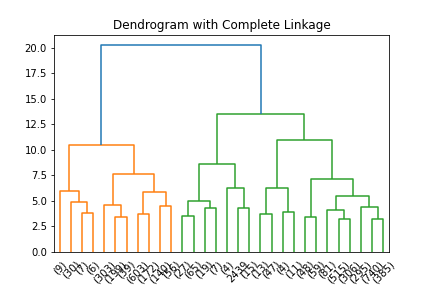
\includegraphics[width=0.65\textwidth]{img/clustering/complete_link.png}
        \caption{\emph{Complete Link}}
        \label{fig:complete_link}
    \end{subfigure}
    \begin{subfigure}{0.49\textwidth}
        \centering
        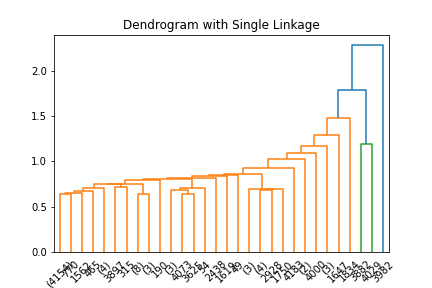
\includegraphics[width=0.65\textwidth]{img/clustering/single_link.png}
        \caption{\emph{Single Link}}
        \label{fig:single_link}
    \end{subfigure}
    \begin{subfigure}{0.49\textwidth}
        \centering
        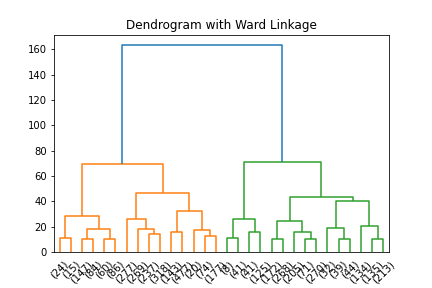
\includegraphics[width=0.65\textwidth]{img/clustering/ward_link.png}
        \caption{\emph{Ward Link}}
        \label{fig:ward_link}
    \end{subfigure}
    \begin{subfigure}{0.49\textwidth}
         \centering
         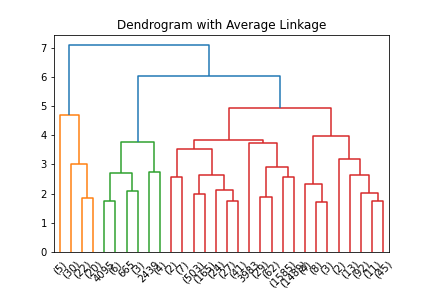
\includegraphics[width=0.65\textwidth]{img/clustering/avg_link.png}
         \caption{\emph{Average Link}}
         \label{fig:avg_link}
     \end{subfigure}
     \caption{Dendograms}
    \label{fig:dendograms}
\end{figure}

\newpage

\subsection{DBSCAN}

We explored different combinations of \emph{eps} for a given \emph{MinPts}; to choose \emph{eps} we checked the \emph{KNN} distance, with $K$ equal to \emph{MinPts}.\\
If \emph{MinPts} is $20$, the optimal \emph{eps} is around $0.25$; in this case, the algorithm found a large dense area surrounded by noisy points, as is showed in Figure \ref{fig:dbscan_good}. By increasing \emph{eps} to $0.3$ the results are the same, if instead we use the value of $0.2$, the algorithm finds more clusters of negligible dimension.

\begin{figure}[h!]
	\vspace{-4mm}
	\captionsetup{justification=centering}
	\centering
	\begin{subfigure}{0.49\textwidth}
		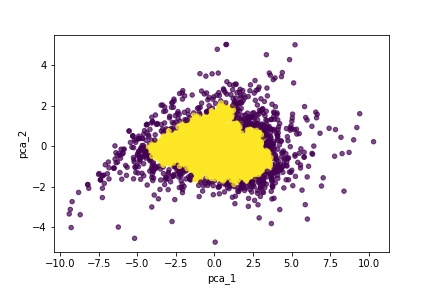
\includegraphics[width=.65\textwidth]{img/clustering/dbscan.png}
		\centering
		\caption{\emph{eps}$ = 0.25$}
		\label{fig:dbscan_good}
	\end{subfigure}
	\begin{subfigure}{0.49\textwidth}
		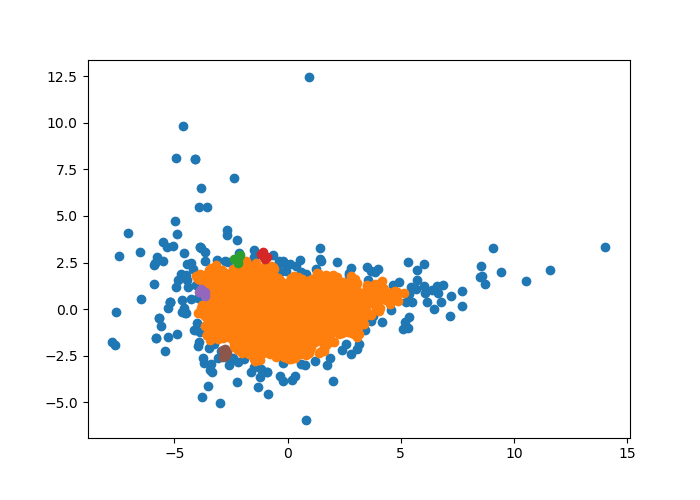
\includegraphics[width=.65\textwidth]{img/clustering/dbscan_bad.png}
		\centering
		\caption{\emph{eps}$ = 0.2$}
		\label{fig:dbscan_bad}
	\end{subfigure}
	\caption{Results of DBSCAN}
	\label{fig:dbscan}
\end{figure}

\subsection{Other clustering}

\begin{wrapfigure}[7]{r}{0.3\textwidth}
	\vspace*{-1cm}
	\begin{center}
		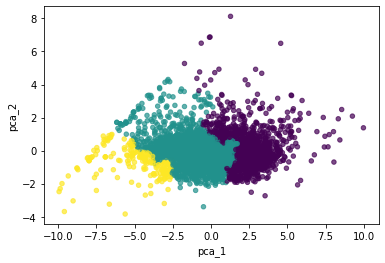
\includegraphics[width=0.25\textwidth]{img/clustering/clust_birch.png}
	\end{center}
	\caption{\emph{Birch} results}
	\label{fig:clust_birch}
\end{wrapfigure}

Together with the previous algorithms, we also tried to run \emph{Fuzzy C-Means} and \emph{Birch}. They both generates a good partitioning, in particular \emph{Fuzzy C-Means} result's resemble the \emph{K-Means} clustering. However the silhouette score is \emph{0.38}, slightly lower than \emph{K-Means}.

\begin{figure}[h!]
     \captionsetup{justification=centering}		
     \centering
     \begin{subfigure}{0.39\textwidth}
         \centering
	 \captionsetup{type=figure}
         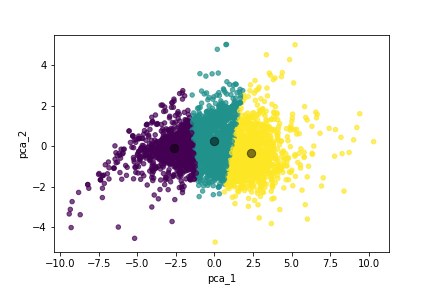
\includegraphics[width=0.8\textwidth]{img/clustering/clust_fcmeans.png}
         \caption{SSE}
         \label{fig:clust_fcmeans}
     \end{subfigure}
     \begin{subfigure}{0.39\textwidth}
         \centering
         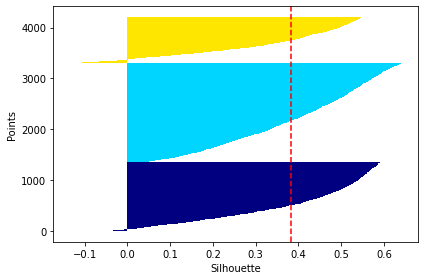
\includegraphics[width=0.8\textwidth]{img/clustering/sil_fcmeans.png}
         \caption{Average silhouette}
         \label{fig:sil_fcmeans}
     \end{subfigure}
     \caption{\emph{Fuzzy C-Means} results}
    \label{fig:fc_means}
\end{figure}

For what concerns \emph{Birch} result's, we have that, even in this case, the algorithm is able to partition the customers into three categories but it generates unbalanced classes. In fact the clusters' cardinalities are \emph{188}, \emph{1315} and \emph{2703}.

\newpage

\subsection{Clustering results}

In conclusion, we opted for the \emph{K-Means} clustering to characterize the customers. As is shown in Figure \ref{fig:pairplot}, the algorithm is able to identify three class of customers corresponding to the low, medium and high spending customers.

\begin{figure}[h!]
	\captionsetup{justification=centering}
	\centering
	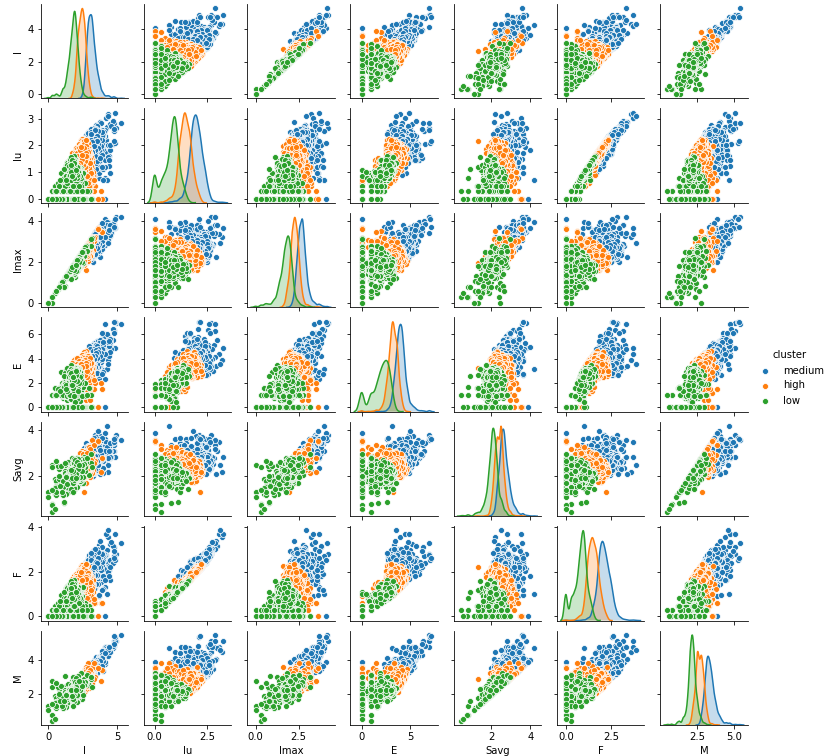
\includegraphics[width=0.85\textwidth]{img/clustering/pair_plot_clust.png}
	\centering
	\caption{K-Means results}
	\label{fig:pairplot}
\end{figure}


%\begin{figure}[h!]
%     \captionsetup{justification=centering}		
%     \centering
%     \begin{subfigure}{0.49\textwidth}
%         \centering
%	 \captionsetup{type=figure}
%         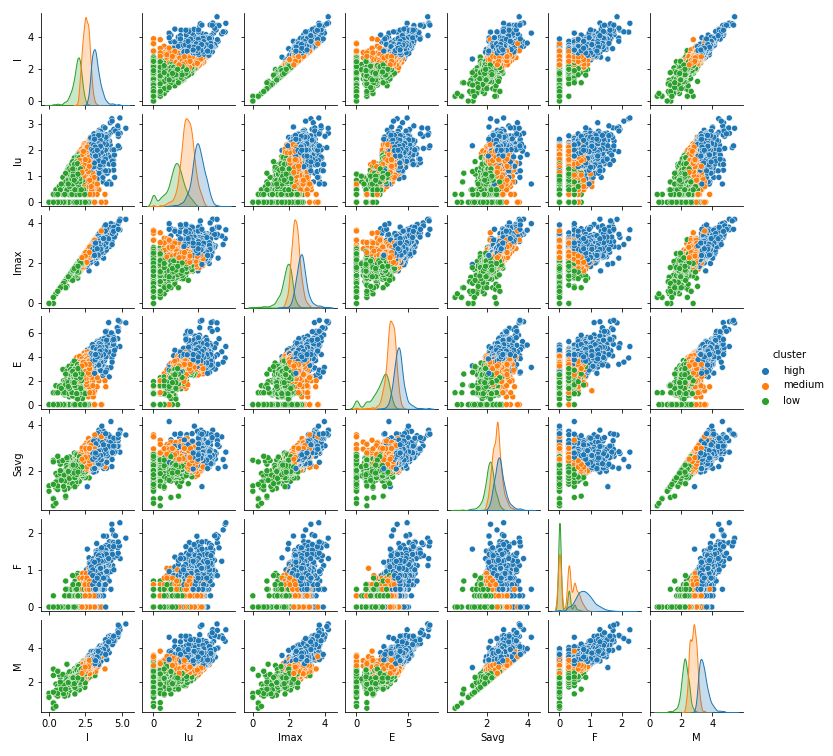
\includegraphics[width=\textwidth]{img/clustering/pairplot_fcmeans.png}
%         \caption{\emph{Fuzzy C-Means}}
%         \label{fig:pplot_fcmeans}
%     \end{subfigure}
%     \begin{subfigure}{0.49\textwidth}
%         \centering
%         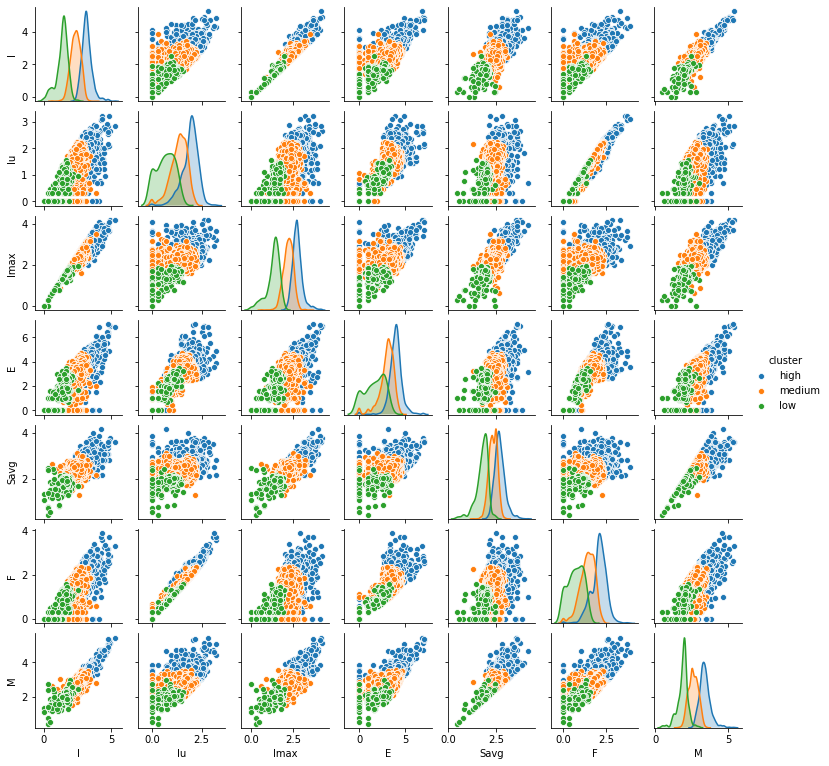
\includegraphics[width=\textwidth]{img/clustering/pairplot_birch.png}
%         \caption{\emph{Birch}}
%         \label{fig:spplot_birch}
%     \end{subfigure}
%     \caption{Clustering pariplots}
   % \label{fig:pplots_extra}
%\end{figure}



